% template adapted from https://github.com/jgm/pandoc-templates/blob/master/default.latex
%%%%%%%%%%%%%%%%%%%%%%%%%%%%%%%%%%%%%%%%%%%%%%%%%%%%%%%%%%%%%%%%%%%%%%%%%%%%%%%%%%%%%%%%%

% Options for packages loaded elsewhere
\PassOptionsToPackage{unicode=true}{hyperref} 
\PassOptionsToPackage{hyphens}{url}
  \PassOptionsToPackage{dvipsnames,svgnames*,x11names*}{xcolor}


\documentclass[
  11pt,
  french,
  A4paper,
  extrafontsizes,onecolumn,openright
  ]{memoir}

% Font family: lmodern by default
\usepackage{fontspec}
  \usepackage{lmodern}

% Double (or whatever) spacing

\usepackage{amssymb, amsmath}
\usepackage{ifxetex,ifluatex}
\usepackage{fixltx2e} % provides \textsubscript

% mathspec: arbitrary math fonts
  \usepackage{unicode-math}
\defaultfontfeatures{Ligatures=TeX,Scale=MatchLowercase}

% More font families
% Main font
% Specific sanserif font
% Specific monotype font
% Specific math font
% Chinese, Japanese, Corean fonts 

% Use upquote if available, for straight quotes in verbatim environments
\IfFileExists{upquote.sty}{\usepackage{upquote}}{}
% Use microtype if available
\IfFileExists{microtype.sty}{%
\usepackage[]{microtype}
\UseMicrotypeSet[protrusion]{basicmath} % disable protrusion for tt fonts
}{}

% Verbatim in note
  \usepackage{fancyvrb}

\usepackage{xcolor}

\usepackage{hyperref}
\hypersetup{
            pdftitle={Statistiques Spatiales},
            pdfauthor={Eric Marcon},
            pdfkeywords={Keyword in English, As a list},
            colorlinks=true,
            linkcolor=Maroon,
            citecolor=Blue,
            urlcolor=Blue,
            breaklinks=true}
            
% Don't use monospace font for urls
\urlstyle{same}  

  \VerbatimFootnotes % allows verbatim text in footnotes

% Geometry package

% Listings package


\usepackage{color}
\usepackage{fancyvrb}
\newcommand{\VerbBar}{|}
\newcommand{\VERB}{\Verb[commandchars=\\\{\}]}
\DefineVerbatimEnvironment{Highlighting}{Verbatim}{commandchars=\\\{\}}
% Add ',fontsize=\small' for more characters per line
\usepackage{framed}
\definecolor{shadecolor}{RGB}{248,248,248}
\newenvironment{Shaded}{\begin{snugshade}}{\end{snugshade}}
\newcommand{\KeywordTok}[1]{\textcolor[rgb]{0.13,0.29,0.53}{\textbf{#1}}}
\newcommand{\DataTypeTok}[1]{\textcolor[rgb]{0.13,0.29,0.53}{#1}}
\newcommand{\DecValTok}[1]{\textcolor[rgb]{0.00,0.00,0.81}{#1}}
\newcommand{\BaseNTok}[1]{\textcolor[rgb]{0.00,0.00,0.81}{#1}}
\newcommand{\FloatTok}[1]{\textcolor[rgb]{0.00,0.00,0.81}{#1}}
\newcommand{\ConstantTok}[1]{\textcolor[rgb]{0.00,0.00,0.00}{#1}}
\newcommand{\CharTok}[1]{\textcolor[rgb]{0.31,0.60,0.02}{#1}}
\newcommand{\SpecialCharTok}[1]{\textcolor[rgb]{0.00,0.00,0.00}{#1}}
\newcommand{\StringTok}[1]{\textcolor[rgb]{0.31,0.60,0.02}{#1}}
\newcommand{\VerbatimStringTok}[1]{\textcolor[rgb]{0.31,0.60,0.02}{#1}}
\newcommand{\SpecialStringTok}[1]{\textcolor[rgb]{0.31,0.60,0.02}{#1}}
\newcommand{\ImportTok}[1]{#1}
\newcommand{\CommentTok}[1]{\textcolor[rgb]{0.56,0.35,0.01}{\textit{#1}}}
\newcommand{\DocumentationTok}[1]{\textcolor[rgb]{0.56,0.35,0.01}{\textbf{\textit{#1}}}}
\newcommand{\AnnotationTok}[1]{\textcolor[rgb]{0.56,0.35,0.01}{\textbf{\textit{#1}}}}
\newcommand{\CommentVarTok}[1]{\textcolor[rgb]{0.56,0.35,0.01}{\textbf{\textit{#1}}}}
\newcommand{\OtherTok}[1]{\textcolor[rgb]{0.56,0.35,0.01}{#1}}
\newcommand{\FunctionTok}[1]{\textcolor[rgb]{0.00,0.00,0.00}{#1}}
\newcommand{\VariableTok}[1]{\textcolor[rgb]{0.00,0.00,0.00}{#1}}
\newcommand{\ControlFlowTok}[1]{\textcolor[rgb]{0.13,0.29,0.53}{\textbf{#1}}}
\newcommand{\OperatorTok}[1]{\textcolor[rgb]{0.81,0.36,0.00}{\textbf{#1}}}
\newcommand{\BuiltInTok}[1]{#1}
\newcommand{\ExtensionTok}[1]{#1}
\newcommand{\PreprocessorTok}[1]{\textcolor[rgb]{0.56,0.35,0.01}{\textit{#1}}}
\newcommand{\AttributeTok}[1]{\textcolor[rgb]{0.77,0.63,0.00}{#1}}
\newcommand{\RegionMarkerTok}[1]{#1}
\newcommand{\InformationTok}[1]{\textcolor[rgb]{0.56,0.35,0.01}{\textbf{\textit{#1}}}}
\newcommand{\WarningTok}[1]{\textcolor[rgb]{0.56,0.35,0.01}{\textbf{\textit{#1}}}}
\newcommand{\AlertTok}[1]{\textcolor[rgb]{0.94,0.16,0.16}{#1}}
\newcommand{\ErrorTok}[1]{\textcolor[rgb]{0.64,0.00,0.00}{\textbf{#1}}}
\newcommand{\NormalTok}[1]{#1}

% Tables
  \usepackage{longtable,booktabs}
  % Fix footnotes in tables (requires footnote package)
  \IfFileExists{footnote.sty}{\usepackage{footnote}\makesavenoteenv{longtable}}{}

% Graphics
  \usepackage{graphicx,grffile}
  \graphicspath{{images/}}
  \makeatletter
  \def\maxwidth{\ifdim\Gin@nat@width>\linewidth\linewidth\else\Gin@nat@width\fi}
  \def\maxheight{\ifdim\Gin@nat@height>\textheight\textheight\else\Gin@nat@height\fi}
  \makeatother
  % Scale images if necessary, so that they will not overflow the page
  % margins by default, and it is still possible to overwrite the defaults
  % using explicit options in \includegraphics[width, height, ...]{}
  \setkeys{Gin}{width=\maxwidth,height=\maxheight,keepaspectratio}



\setlength{\emergencystretch}{3em}  % prevent overfull lines
\providecommand{\tightlist}{%
  \setlength{\itemsep}{0pt}\setlength{\parskip}{0pt}}

  \setcounter{secnumdepth}{5}

% set default figure placement to htbp
\makeatletter
\def\fps@figure{htbp}
\makeatother

% Include headers (preamble.tex) here
%%% Complete the preamble of the LaTeX template
%%%------------------------------------------------------------------------------

%%% PACKAGES 
\usepackage{lipsum} % Dummy text.

\usepackage{enumitem}

  % load polyglossia as late as possible as it *could* call bidi if RTL lang (e.g. Hebrew or Arabic)
  \usepackage{polyglossia}
  \setmainlanguage[]{french}
  \setotherlanguage[variant=american]{english}
  \setotherlanguage[variant=british]{english}
  \setotherlanguage[]{french}




\usepackage[style=authoryear-ibid,backend=bibtex,citestyle=verbose-inote,pageref=true,isbn=false,backref=true,giveninits=true,uniquename=init,maxcitenames=2,maxbibnames=150,sorting=nyt,sortcites=false]{biblatex}
\addbibresource{../Library.bib}
\addbibresource{packages.bib}

% Specific commands for EcoFoG style. Must come after biblatex.
\usepackage{latex/BookTemplate}


% Title, author, etc. from YAML to LaTeX
%%%%%%%%%%%%%%%%%%%%%%%%%%%%%%%%%%%%%%%%%%%%%%%%%%%%%%%%%%

\title{Statistiques Spatiales}


\author{Eric Marcon}


\date{2017-12-21}


% Main title page with filigrane
%%%%%%%%%%%%%%%%%%%%%%%%%%%%%%%%%%%%%%%%%%%%%%%%%%%%%%%%%%
\newcommand{\MainTitlePage}[1][]{
	\SmallMargins % Margins
	\pagestyle{empty} % No header/footer
	~\\ % Print a character or the page will not exist
	\begin{textblock}{2}(30,10)
		\rule{1pt}{\paperheight-20mm}
	\end{textblock} 
	\begin{textblock}{140}(50, 45)
		\flushright 
		\begin{Spacing}{3}
			{\fontsize{45}{45}\selectfont \thetitle\par}
		\end{Spacing}
	\end{textblock}
	\begin{textblock}{140}(50, 125)
		\flushright 
		{\fontfamily{qtm}\Large \theauthor}
	\end{textblock} 
	\begin{textblock}{120}[1, 1](225, 297)
		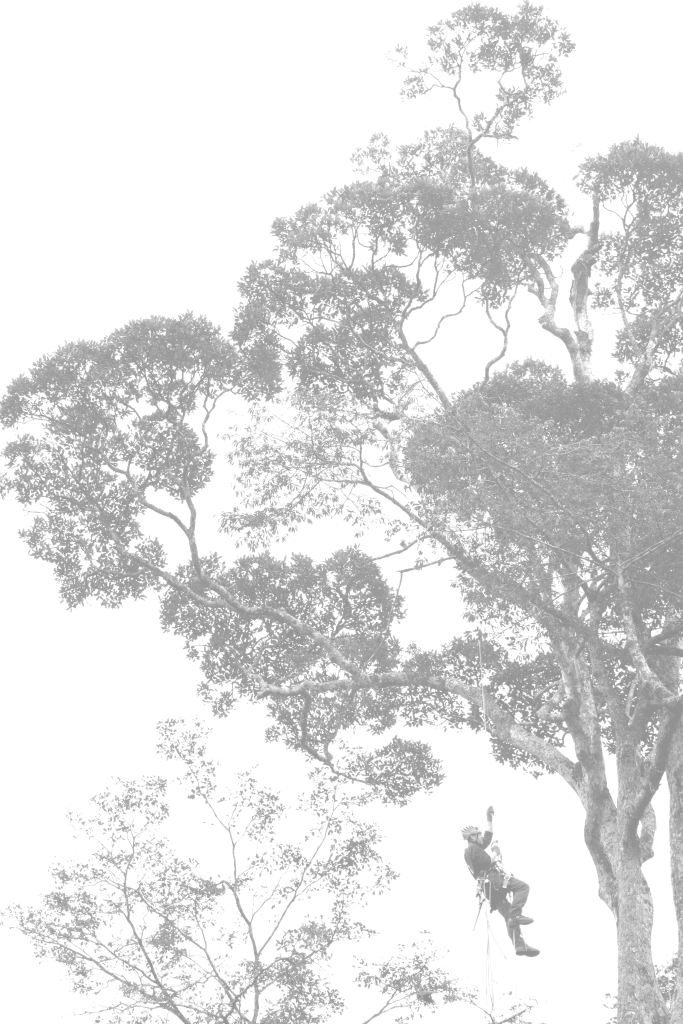
\includegraphics[width=10cm]{Filigrane}
	 \end{textblock} 
	\begin{textblock}{140}[0, 1](50, 262)
		\normalfont	Version: \thedate
	\end{textblock} 
	\newpage
	~\\ % Print a character or the page will not exist
	\begin{textblock}{140}(40, 40)
		#1
	\end{textblock}
	\begin{textblock}{140}[0,1](40, 270)
		\centering
    \includegraphics[width=5cm]{Logo-Lab}\\ \bigskip
		UMR \'Ecologie des forêts de Guyane\\
		\url{http://www.ecofog.gf}\\[3\baselineskip]
		Les opinions émises par les auteurs sont personnelles et n’engagent ni l’UMR EcoFoG ni ses tutelles.
    
    \tiny{Photographie en couverture: Hadrien Lalagüe}
	\end{textblock}
	\newpage
}

% PhD / HDR Thesis
%%%%%%%%%%%%%%%%%%%%%%%%%%%%%%%%%%%%%%%%%%%%%%%%%%%%%%%%%%


% End of preamble
%%%%%%%%%%%%%%%%%%%%%%%%%%%%%%%%%%%%%%%%%%%%%%%%%%%%%%%%%%


\usepackage{amsthm}
\newtheorem{theorem}{Theorem}[chapter]
\newtheorem{lemma}{Lemma}[chapter]
\theoremstyle{definition}
\newtheorem{definition}{Definition}[chapter]
\newtheorem{corollary}{Corollary}[chapter]
\newtheorem{proposition}{Proposition}[chapter]
\theoremstyle{definition}
\newtheorem{example}{Example}[chapter]
\theoremstyle{definition}
\newtheorem{exercise}{Exercise}[chapter]
\theoremstyle{remark}
\newtheorem*{remark}{Remark}
\newtheorem*{solution}{Solution}
\begin{document}
\frontmatter

% Title page
%%%%%%%%%%%%%%%%%%%%%%%%%%%%%%%%%%%%%%%%%%%%%%%%%%%%%%%%%%

\MainTitlePage[Ce document est réalisé de façon dynamique et reproductible grâce à:

\begin{itemize}
  \item \LaTeX, dans sa distribution Miktex (\url{http://miktex.org/}) et la classe memoir (\url{http://www.ctan.org/pkg/memoir}).
  \item R (\url{http://www.r-project.org/}) et RStudio (\url{http://www.rstudio.com/})
  \item bookdown. (\url{http://bookdown.org/})
\end{itemize}]





% Before Body
%%%%%%%%%%%%%%%%%%%%%%%%%%%%%%%%%%%%%%%%%%%%%%%%%%%%%%%%%%




% Contents
%%%%%%%%%%%%%%%%%%%%%%%%%%%%%%%%%%%%%%%%%%%%%%%%%%%%%%%%%%

\LargeMargins
{
\hypersetup{linkcolor=}
\setcounter{tocdepth}{3}
\tableofcontents
}


% Body
%%%%%%%%%%%%%%%%%%%%%%%%%%%%%%%%%%%%%%%%%%%%%%%%%%%%%%%%%%

\LargeMargins
\chapter*{Introduction}\label{introduction}
\addcontentsline{toc}{chapter}{Introduction}

Pourquoi étudier les structures spatiales ?

L'analyse des structures spatiales peut être considérée tout d'abord
comme un outil statistique élémentaire. Quand on observe une carte sur
laquelle sont placés des objets, ils ne semblent en général pas répartis
au hasard. On peut voir des variations de densité, sous la forme de
gradients ou d'agrégats. Pour décrire un phénomène quantitatif à partir
d'un certain nombre d'observations, disons le diamètre moyen des arbres
d'un peuplement, on utilise classiquement l'outil fourni par la théorie
des variables aléatoires : on mesure un certain nombre d'arbres, on
considère que leur diamètre moyen est un estimateur de l'espérance de la
variable aléatoire qu'est le diamètre de chaque arbre, et on calcule la
variance de l'échantillon pour avoir une idée de la variabilité des
diamètres. Si on s'intéresse maintenant à la répartition spatiale de ces
arbres, la quantité d'information disponible est bien plus importante :
la densité des arbres, leur diamètre moyen selon le lieu et les
interactions éventuelles des arbres entre eux. Les outils mathématiques
nécessaires sont les processus ponctuels, généralisation spatialisée
(généralement à deux dimensions) des variables aléatoires.

La question fondamentale consiste à caractériser clairement ce qu'on
observe. Prenons l'exemple d'un peuplement forestier dans lequel les
arbres d'une espèce sont apparemment regroupés et forment des agrégats.
Deux causes peuvent en être responsables : l'hétérogénéité du milieu
favorise la présence de cette espèce localement, la densité des arbres
est alors variable, ou bien les arbres sont regroupés par des processus
d'agrégation (par exemple une faible dispersion des graines)
indépendamment du milieu qu'on supposera dans ce cas homogène. Les
mécanismes écologiques sont extrêmement différents dans les deux cas.
Mais la distinction entre hétérogénéité et agrégation est formellement
impossible sur un jeu de données unique : des hypothèses de travail sont
indispensables. Cette difficulté est probablement la raison pour
laquelle de nombreuses méthodes statistiques ont été mises en place pour
détecter les structures spatiales. Une revue complète en sera faite
(chapitre TODO), la famille d'outils la plus efficace sera étudiée en
détail (chapitre TODO) ainsi que ses fondements mathématiques (les
processus ponctuels, chapitre \ref{Processus}) et de nouveaux outils
seront proposés pour repousser les limites actuelles. La relation
directe entre les processus ponctuels et les phénomènes écologiques
sous-jacents est difficile, à cause de la simplification excessive mais
surtout parce que la réalisation d'un processus observée sous la forme
d'un semis de points est instantanée et unique alors qu'un peuplement
forestier est le résultat d'une histoire et de processus successifs.

La théorie des processus ponctuels est indispensable pour comprendre les
méthodes présentées ici. Une présentation en est faite dans premier
chapitre. Le deuxième chapitre présente l'état de l'art en termes
d'analyse spatiale des processus ponctuels suivi de l'introduction de
nouveaux outils permettant d'étendre son champ d'application. L'objectif
est de permettre la caractérisation des structures spatiales dans un
cadre théorique aussi vaste que possible et répondant aux exigences des
données réelles, comme la prise en compte de l'hétérogénéité.

\mainmatter

\chapter{Processus classiques}\label{Processus}

Les processus ponctuels fournissent le cadre mathématique nécessaire à
l'étude des structures spatiales. Une définition mathématique est
nécessaire avant de présenter les processus les plus courants, dont le
processus de Poisson. L'approche utilisée classiquement par les
non-mathématiciens est locale : les propriétés d'un processus sont
définies autour de chaque point. Elle a l'avantage d'être concrète et
facilement compréhensible. Son inconvénient est de laisser un certain
flou sur le comportement global du processus. Une définition globale est
nécessaire pour aller plus loin : c'est celle que nous présenterons en
première partie de ce chapitre. La définition locale est présentée
en-suite pour les lecteurs rebutés par les équations.

Ensuite, nous analyserons en détail quelques processus classiques,
choisis pour leur utilité en écologie puis les méthodes nécessaires à
leur simulation.

\section{Définitions}\label{definitions}

\subsection{Processus ponctuel}\label{processus-ponctuel}

Nous nous placerons dans une partie du plan, typiquement une placette
forestière, notée \(A\), \(A \subset R^2\). Les définitions données ici
et la plupart des résultats sont valables dans un espace de dimension
quelconque finie mais on se limitera en pratique à un espace à deux
dimensions. D'autre part, travailler sur une placette de taille infinie
n'a pas d'intérêt pratique, mais rien ne s'y opposerait sur le plan
mathématique, sauf dans certains cas qui seront précisés dans le texte.
\(A\) sera appelée aire ou zone ou fenêtre d'étude.

Nous nous intéresserons à des ensembles dénombrables de points (on dira
aussi ``semis de points''). Les points seront notés en minuscules, les
ensembles en majuscules : \(X \subset R^2\) , \(x \in X\). Le semis de
point \(X\) sera généralement défini sur tout le plan, et son nombre de
points sera infini. À l'intérieur de l'aire d'étude \(A\), un sous
ensemble de \(X\) noté \(X_A\) sera observé et cartographié :
\(X_A = X \cap A\). Nous ne nous intéresserons qu'à des ensembles de
points localement finis, c'est-à-dire tels que leur nombre de points
dans \(A\) soit fini : \(n(A) < \infty\) pour \(A\) borné. Cette
restriction n'a pas de conséquences pratiques. Il est impossible de
définir directement une fonction qui attribuerait à chaque semis la
probabilité de le tirer, parce que la probabilité de chaque semis est
nulle. On passe donc par des ensembles de semis de points, dont la
probabilité n'est pas nulle. L'ensemble des semis de points localement
finis est noté \(N_f\). \(N_f\) peut être équipé d'une
\(\sigma\)-algèbre \(\mathcal{N_f}\). Les éléments \(F\) de
\(\mathcal{N_f}\) sont des ensembles de semis de points localement
finis. \(\mathcal{N_f}\) est une tribu (ou \(\sigma\)-algèbre) de \$
N\_\$f :

\begin{itemize}
  \item l'ensemble vide appartient à $\mathcal{N_f}$;
  \item pour tout $F \in \mathcal{N_f}$, le complémentaire de $F$ dans $\mathcal{N_f}$ appartient aussi à $\mathcal{N_f}$;
  \item L’union de $(F_1, F_2, F_3,…)$, une suite dénombrable d'éléments de $\mathcal{N_f}$ appartient aussi à $\mathcal{N_f}$.
\end{itemize}

\((N_f, \mathcal{N_f})\) est un espace probabilisable. Il reste à le
doter d'une mesure \(P\), la probabilité de tirer un ensemble de semis
de points particulier \(F\). Cet ensemble est défini par le nombre de
points tirés, \(N(A)\), pour tout \(A\) borné. \(P\) est une mesure car
:

\begin{itemize}
  \item $P(\emptyset)=0$
  \item P est $\sigma$-additive : $P(\bigcup_(i=1)^n F_i) = \sum_(i=n)^n {P(F_i)}$, où $\bigcup_(i=1)^n F_i$ est une union disjointe.
\end{itemize}

\(P\) est une probabilité car on fixe \(P(\mathcal{N_f})=1\).

Un processus ponctuel est défini comme une application d'un espace de
probabilité \((\Omega, F, P)\) vers \((N_f,\mathcal{N_f})\) tel que
\(N(A)\) est une variable aléatoire pour tout \(A\) borné. La définition
précise de \((\Omega, F, P)\) importe peu puisqu'il est impossible à
utiliser directement. Les processus sont notés en lettres grecques
majuscules, par exemple \(\Xi\). Un semis de points X est une
réalisation de \(Xi\). On note \(P(X \in F)\) la probabilité que le
tirage de \(\Xi\) soit un élément d'un ensemble de semis de points \(F\)
particulier, par exemple défini par son nombre de points. Enfin, les
surfaces comme \(\|A\|\) seront notées abusivement \(A\) pour alléger
les équations.

\subsection{Propriété de premier
ordre}\label{propriete-de-premier-ordre}

Soit \(S\) une partie de \(A\). La propriété de premier ordre
\(\mu(S)\), appelée également mesure d'intensité du processus \(\Xi\),
est l'espérance du nombre de points dans \(S\) :

\begin{equation}
  \mu(S)=E(N(S))
\end{equation}

Dans tous les cas que nous traiterons, la mesure d'intensité pourra être
écrite comme l'intégrale d'une fonction d'intensité \(\lambda\) :

\begin{equation}
  \mu(S)=\int_S \lambda(x)dx
\end{equation}

\subsection{Propriété de second ordre}\label{propriete-de-second-ordre}

La mesure du moment factoriel de second ordre de deux parties de \(A\),
\(S_1\) et \(S_2\), est l'espérance du nombre de paires de points du
processus \(\Xi\) se trouvant respectivement dans \(S_1\) et S\(_2\) :

\begin{equation}
  \mu_2(S_1,S_2 ) = E \left(\sum_{x_1 ,x_2 \in X, x_1 \ne x_2}{1(x_1 \in S_1, x_2 \in S_2)} \right)
\end{equation}

De même, cette mesure pourra être écrite comme l'intégrale de
\(\lambda_2\), appelée densité du produit de second ordre :

\begin{equation}
  \mu_2 S_1,S_2 ) = \iint_{(R^2)^2}{1(x_1 \in S_1, x_2 \in S_2) \lambda_2(x_1, x_2)dx_1 dx_2}
\end{equation}

On peut démontrer \autocite{Moller2004} que :
\[ E(N(S_1 )N(S_2 )) = \lambda_2(S_1,S_2)+\lambda(S_1 \cap S_2)\]

\section{Définition locale}\label{definition-locale}

Un processus ponctuel est l'équivalent d'une variable aléatoire dont le
résultat est un ensemble de points noté \(X\), dans un ensemble de
réalisations possibles, qui sera toujours ici une surface connue et
délimitée notée \(A\).

On utilise les processus ponctuels comme outils mathématiques pour
caractériser et éventuellement modéliser des événements dont on connaît
la répartition spatiale, par exemple les arbres dans une forêt. Une
façon intéressante de décrire un processus ponctuel dont on ne connaît
pas la loi consiste à utiliser ses propriétés de premier ordre et de
second ordre.

\section{Processus de Poisson
homogène}\label{processus-de-poisson-homogene}

Le processus de Poisson est un processus stationnaire et isotrope, dont
la réalisation donne des points à la position complètement aléatoire.
Inversement, un processus ponctuel complètement aléatoire est un
processus de Poisson \autocite[démonstration :][pp.~51-52]{Diggle1983}.

Le processus de Poisson joue un rôle central en statistiques spatiales,
à la fois parce que c'est le plus simple donc celui dont les propriétés
ont été le mieux étudiées, et aussi parce qu'il constitue généralement
le modèle nul contre lequel des semis de points peuvent être testés.
C'est un processus à accroissements indépendants, il joue le rôle des
marches aléatoires pour les séries temporelles à temps discret et du
mouvement Brownien pour les séries à temps continu. Ces propriétés sont
utilisées pour le calcul de l'intervalle de confiance de la fonction
\emph{K} de Ripley.

\section{Propriété de premier ordre}\label{propriete-de-premier-ordre-1}

Une réalisation d'un processus de Poisson de paramètre \(\lambda A\) sur
l'aire d'étude A est un semis de points complètement aléatoire
d'intensité \(\lambda\). Le nombre de points suit une loi de Poisson de
paramètre \(\lambda A\), c'est-à-dire que :

\begin{equation}
  P(n(A)=k) = e^{-\lambda A} \frac{(\lambda A)^k}{k!}.
  \label{eq:Poisson}
\end{equation}

La simulation d'un processus de Poisson (figure \ref{fig:Poisson}) est
faite par la commande \texttt{rpoispp} de \emph{spatstat}.

\begin{Shaded}
\begin{Highlighting}[]
\NormalTok{X <-}\KeywordTok{rpoispp}\NormalTok{(}\DataTypeTok{lambda=}\DecValTok{1}\NormalTok{, }\DataTypeTok{win=}\KeywordTok{as.owin}\NormalTok{(}\KeywordTok{c}\NormalTok{(}\DecValTok{0}\NormalTok{, }\DecValTok{10}\NormalTok{, }\DecValTok{0}\NormalTok{, }\DecValTok{10}\NormalTok{)))}
\KeywordTok{plot}\NormalTok{(X, }\DataTypeTok{main=}\StringTok{""}\NormalTok{)}
\KeywordTok{axis}\NormalTok{(}\DecValTok{1}\NormalTok{); }\KeywordTok{axis}\NormalTok{(}\DecValTok{2}\NormalTok{)}
\end{Highlighting}
\end{Shaded}

\begin{SCfigure}

{\centering 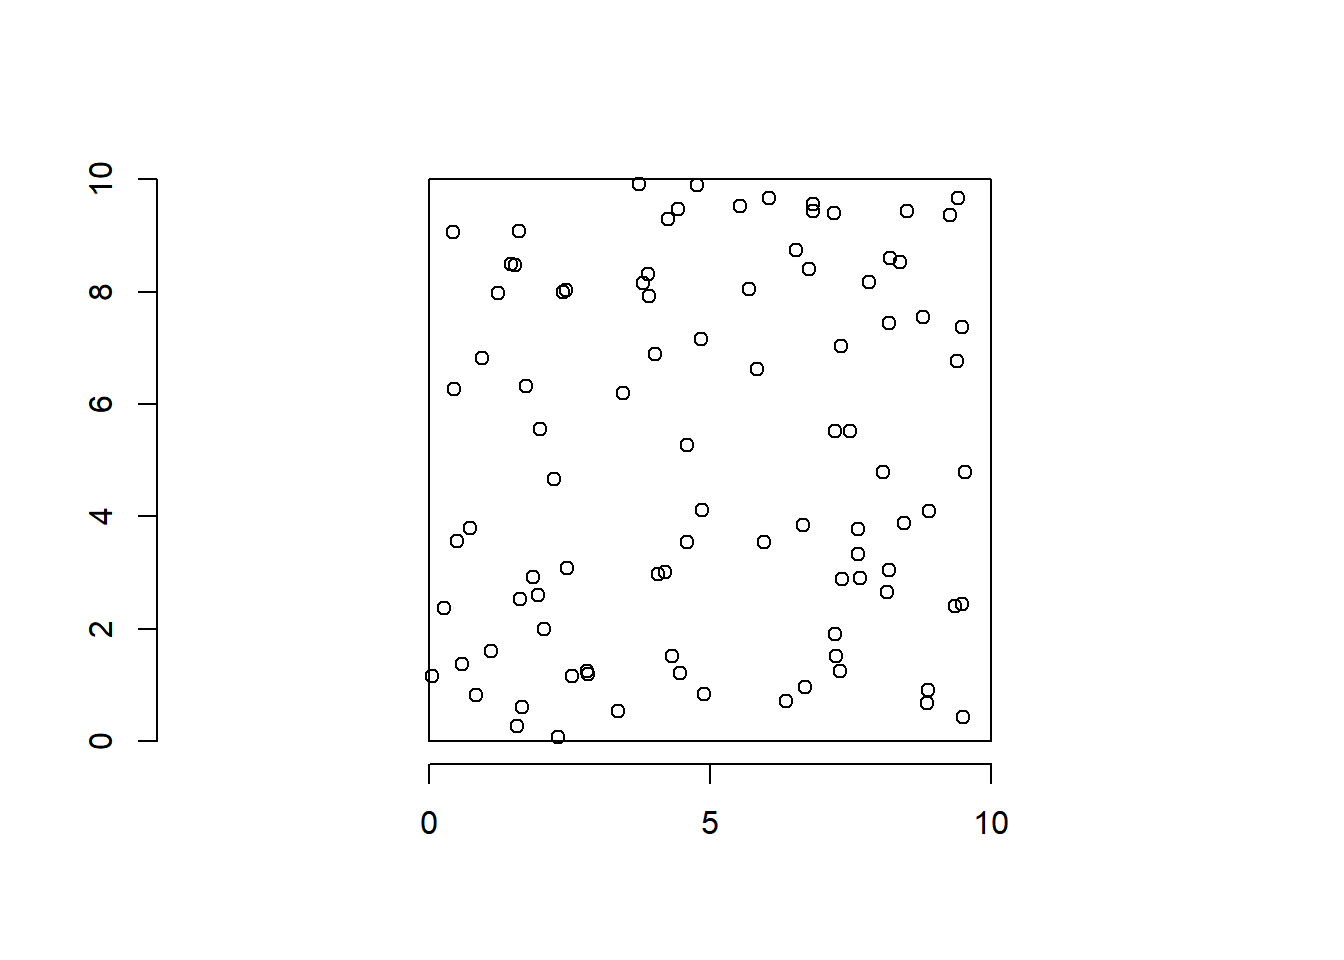
\includegraphics[width=0.8\linewidth]{MyBook_files/figure-latex/Poisson-1} 

}

\caption{Simulation d’un processus de Poisson homogène d’intensité 1}\label{fig:Poisson}
\end{SCfigure}


% Bibliography
%%%%%%%%%%%%%%%%%%%%%%%%%%%%%%%%%%%%%%%%%%%%%%%%%%%%%%%%%%

\backmatter
\SmallMargins

%
\printbibliography


% Tables (of tables, of figures)
%%%%%%%%%%%%%%%%%%%%%%%%%%%%%%%%%%%%%%%%%%%%%%%%%%%%%%%%%%




% After-body (LaTeX code inclusion)
%%%%%%%%%%%%%%%%%%%%%%%%%%%%%%%%%%%%%%%%%%%%%%%%%%%%%%%%%%



% Back cover
%%%%%%%%%%%%%%%%%%%%%%%%%%%%%%%%%%%%%%%%%%%%%%%%%%%%%%%%%%%

% Even page, small margins, no running head, no page number.
\evenpage
\SmallMargins
\thispagestyle{empty}

\begin{normalsize}

\begin{description}

\selectlanguage{french}
\item[Résumé:]
Résumé en Français, en quatrième de couverture.

Lorem ipsum dolor sit amet, consectetuer adipiscing elit. Maecenas
porttitor congue massa. Fusce posuere, magna sed pulvinar ultricies,
purus lectus malesuada libero, sit amet commodo magna eros quis urna.

Nunc viverra imperdiet enim. Fusce est. Vivamus a tellus.

\selectlanguage{french}
\item[Mots clés :]
Mot clé en Français, En liste.
~\\

\selectlanguage{english}
\item[Abstract:]
English abstract, on the last page.

Lorem ipsum dolor sit amet, consectetuer adipiscing elit. Maecenas
porttitor congue massa. Fusce posuere, magna sed pulvinar ultricies,
purus lectus malesuada libero, sit amet commodo magna eros quis urna.

Nunc viverra imperdiet enim. Fusce est. Vivamus a tellus.

\selectlanguage{english}
\item[Keywords:]
Keyword in English, As a list.

\end{description}

\end{normalsize}

\vspace*{\fill}
\centering\includegraphics[width=.3\textwidth]{images/Logo-Lab}
\end{document}
